\section{System Model}
\label{sec:model}
In this section, we elaborate the model of edge computing networks with random job arrivals, uploading latency and computation time,
\hongyc{as well as the signaling mechanism with periodic broadcast.}
% as well as the signaling model with periodic broadcast which introduce the job dispatching actions making under partially observable system state at each AP.
%----------------------------------------------------------------------------------------%
\subsection{Network Model}
\begin{figure*}[htp!]
    \centering
    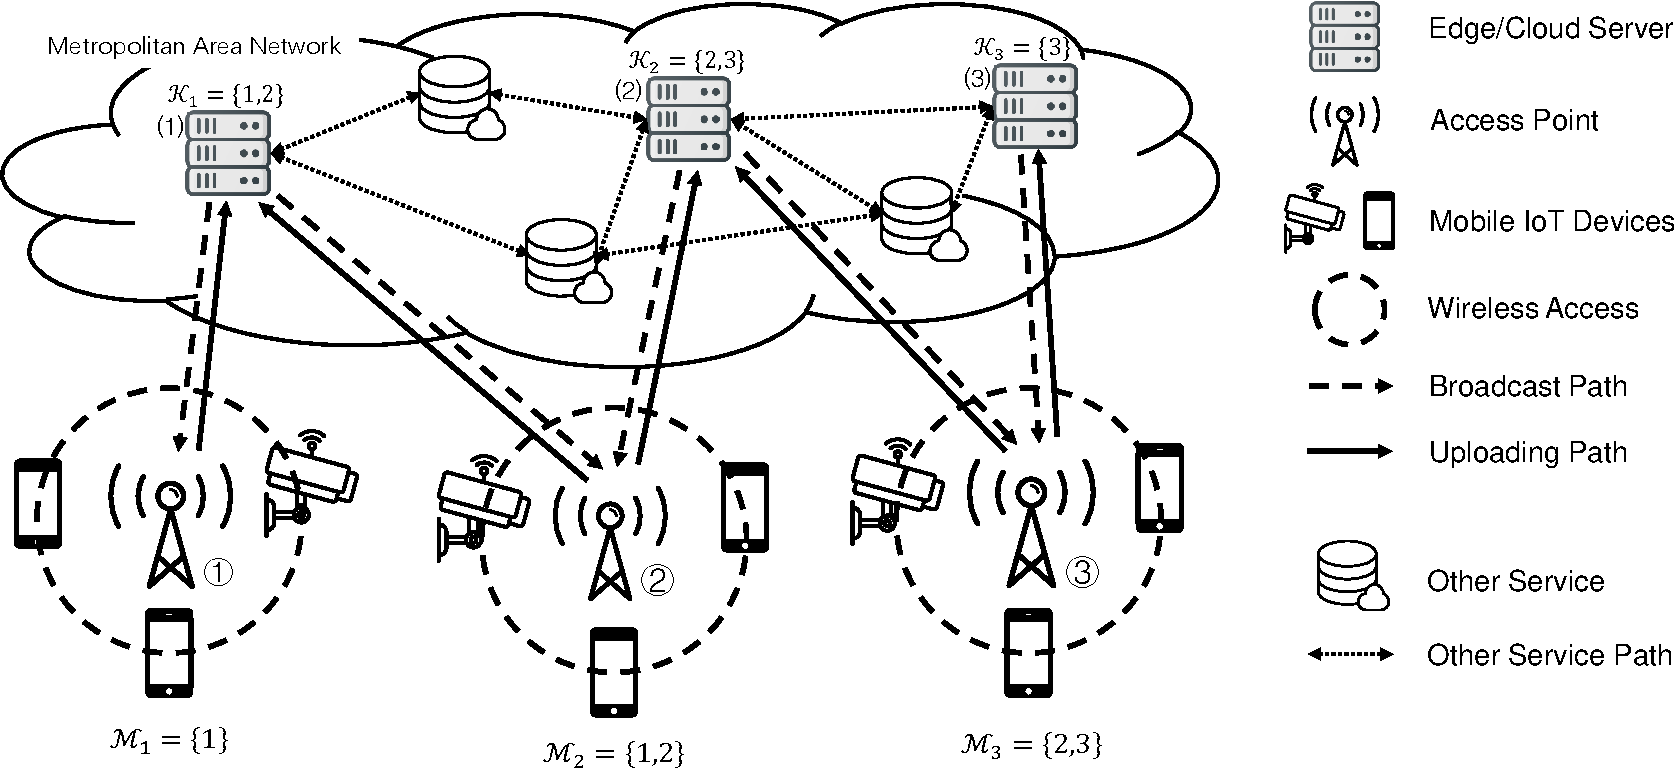
\includegraphics[width=0.60\textwidth]{system-model.pdf}
    \caption{The Illustration of System Model}
    \label{fig:system}
\end{figure*}

We consider an edge computing system with $K$ Access Points (APs) and $M$ edge servers, which are connected in a network as illustrated in Fig.\ref{fig:system}.
The sets of APs and edge servers are denoted as $\apSet \define \set{1,\dots,K}$ and $\esSet \define \set{1,\dots,M}$, respectively.
The communication latency among these APs and edge servers is random.
Each AP collects the computation jobs from the mobile users within its coverage, and makes dispatching action on the processing edge servers for each job.
It is assumed that the $k$-th AP only dispatches the computation jobs to the edge servers within a certain number of hops.
Let $\esSet_{k} \subseteq \esSet$ be the set of edge servers which can compute the jobs from the $k$-th AP, and $\apSet_{m}$ be the set of APs, which may upload jobs to the $m$-th edge server.
We refer to $\esSet_{k}$ as the \emph{candidate server set} of the $k$-th AP, and $\apSet_{m}$ as the \emph{potential AP set} of the $m$-th edge server ($\forall k\in\apSet, m\in\esSet$).
Different APs may have different candidate servers according to their locations in the network, as illustrated in Fig.\ref{fig:system}.
In this edge computing network, each AP and edge server periodically broadcast their state information (the state information is defined in the Section \ref{subsec:broadcast}), and one AP updates its strategy of job dispatching when receiving the broadcast state information.
In this paper, we shall optimize the job dispatching strategy distributed at APs with partially collected state information{, where both job uploading and state information broadcasting suffer from random transmission latency.}

%NOTE: [job space support and arrival process]
\comments{
    Without loss of generality, it is assumed that there are $J$ types of jobs computed in this system, which are denoted via the set $\jSpace \define \set{1,\dots,J}$.
    \hongyc{
        This implies that the resource allocation is fixed for some classified jobs, which is not the concern to optimize in this paper.
        Hence, the dispatcher design in this paper could generalized to any edge-cloud model, with pre-defined resource allocation scheme.
    }
}
The time axis is organized by time slots.
The arrivals of the type-$j$ jobs at the $k$-th AP ($\forall k\in\apSet,j\in\jSpace$) in different time slots are assumed to be independent and identically distributed (i.i.d.) Bernoulli random variables, and the arrival probability is denoted as $\lambda_{k,j}$.
Let $A_{k,j}(t) \in \set{0,1}$ represents the event of job arrival, where $A_{k,j}(t)=1$ means one type-$j$ job arrives at the $k$-th AP in the $t$-th time slot, and $A_{k,j}(t)=0$ means otherwise.
Hence,
\begin{align}
    \Pr\{ A_{k,j}(t) = 1 \} = \lambda_{k,j}, \forall t,k\in\apSet,j\in\jSpace.
\end{align}

%NOTE: [uploading process]
Each AP immediately dispatches each type of received jobs to one edge server.
Different types of jobs may have different distributions of the input data size.
Moreover, due to the random traffic in the network, the job uploading from one AP to one edge server consumes a random number of time slots.
It is assumed that the random uploading latency are independent for each job.
Specifically, let $\mathbb{U}_{k,m,j}(\Xi)$ be the uploading latency distribution of the type-$j$ jobs from the $k$-th AP to the $m$-th edge server with support $\set{1, \dots, \Xi}$ ($\forall k\in\apSet, m\in\esSet, j\in\jSpace$), whose expectation is denoted as $u_{k,m,j}$.

%NOTE: [computation process]
\comments{
    For jobs computation process on edge server, we adopt the \emph{unrelated machines assumption} as in \cite{tan-online} where the computation time on different edge servers would follow independent distribution.
    Furthermore, there are $J$ parallel virtual machines (VMs) running on each edge server for processing the $J$ job types, respectively.
    And we assume that the computation time of different job types on different edge servers follows independent memoryless geometric distribution 
    \footnote{In this paper, we adopt the memoryless geometric distribution to simplify the elaboration of notations. In fact, the proposed algorithm can be easily extended to other distributions.}
    with different expectations \cite{TOWC18-HuangKb}.
}
Let $\mathbb{G}(1/c_{m,j})$ be the distribution of the computation time slots for the type-$j$ jobs on the $m$-th edge server, where $\mathbb{G}$ denotes the geometric distribution, and $c_{m,j}$ is the expectation.
Let $f_{m,j}$ be its probability mass function (PMF), we have
\begin{align}
    f_{m,j}(x) \define (1-\frac{1}{c_{m,j}})^{x-1} \frac{1}{c_{m,j}}.
\end{align}
For each job type, the uploaded jobs are computed in a First-Come-First-Serve (FCFS) manner, and a processing queue with a maximum job number $L_{max}$ is established for each VM.
The arrival jobs will be discarded when the processing queue is full.
%----------------------------------------------------------------------------------------%

\subsection{\comments{Signaling Mechanism with Periodic Broadcast}}
\label{subsec:broadcast}
In order to facilitate distributed dispatching for the APs, \comments{the signling mechanism with periodic broadcast is introduced.}
We refer to every $t_B$ time slots as a broadcast interval.
As illustrated in Fig.\ref{fig:brd-timeline}, at the beginning of each broadcast interval, the local state information (LSI) of APs and edge servers are broadcast, and each AP updates its dispatching strategy of job dispatching when observing the broadcast LSI s from some APs and edge servers.
As a remark notice that the observed LSI may be outdated due to transmission latency among APs and edge servers.
The LSI at the APs and edge servers, global state information, and observed LSI at the APs are defined below.

%NOTE: State and Broadcast Information for AP
\begin{definition}[Local State Information of APs]
    Let $R^{(k)}_{m,j}(\xi,t,n) \in \set{0,1}$ be the indicator of the type-$j$ jobs at the $n$-th time slot of the $t$-th interval.
    Its value is $1$ when there is one job being uploaded from the $k$-th AP to the $m$-th server which has been delivered for $\xi$ time slots, and $0$ otherwise.
    Let $\omega_{k,j}(t)$ be the target processing edge server for the type-$j$ jobs of the $k$-th AP at the very beginning of the $t$-th broadcast interval, and $\omega_{k,j}(t+1)$ be the updated target processing edge server when the $k$-th AP observe a number of the broadcast LSIs of the $t$-th broadcast interval.
    The LSI of the $k$-th AP at the beginning of the $t$-th broadcast interval is defined as
    {\small
    \begin{align}
        \mathcal{R}_{k}(t) \define
        \Paren{
            \Brace{\vec{R}^{(k)}_{m,j}(t,0) \Big| \forall m\in\esSet,j\in\jSpace},
            \mathcal{A}_{k}(t)
        },
    \end{align}
    }
    where
    \begin{align}
        \vec{R}^{(k)}_{m,j}(t,0) \define \Paren{
            R^{(k)}_{m,j}(0,t,0), \dots, R^{(k)}_{m,j}(\Xi,t,0)
        },
    \end{align}
    and
    \begin{align}
        \mathcal{A}_{k}(t) &\define \Brace{\omega_{k,j}(t) \Big| \forall j\in\jSpace}
    \end{align}
    is referred as the dispatching actions of the $k$-th AP at the start of the $t$-th broadcast interval.
\end{definition}

%NOTE: State and Broadcast Information for Edge Server
\begin{definition}[Local State Information of Edge Servers]
    Let $Q_{m,j}({t,n})$ be the number of type-$j$ jobs on the $m$-th edge server at the $n$-th time slot of the $t$-th interval ($\forall m\in\esSet, j\in\jSpace$).
    The LSI of the $m$-th edge server at the $t$-th broadcast interval is defined as
    \begin{align}
        \mathcal{Q}_{m}(t) \define \Brace{
            Q_{m,j}(t, 0) \Big| \forall j\in\jSpace
        }.
    \end{align}
\end{definition}

\begin{definition}[Global State Information]
    The global state information (GSI) of the $t$-th broadcast interval is defined as the aggregation of the broadcast LSIs from all the APs and edge servers, i.e.,
    \begin{align}
        \Stat(t) \define
            \Paren{
                \Brace{\mathcal{R}_{k}(t) \Big| \forall k\in\apSet},
                \Brace{\mathcal{Q}_{m}(t) \Big| \forall m\in\esSet}
            }.
    \end{align}
\end{definition}

%NOTE: Conflict of AP set and partial information definition
As the APs and edge servers may reside in different locations of a MAN, the transmission latency of LSI is not negligible.
It might be inefficient for one AP (say the $k$-th AP) to collect the complete GSI before update the dispatching policy.
For example, the transmission latency of the LSI from the edge servers out of its \emph{candidate server set} $\esSet_{k}$ may be large, and some broadcast information may be discarded by the routers after a certain number of hops.
In this paper, we shall investigate the dispatching design based on the \emph{observed state information} at each AP.
Specifically, the \emph{conflict AP sets} and the \emph{observed state information} are defined below, respectively.
\begin{definition}[Conflict AP Set]
    The conflict AP set to the $k$-th AP consists of the neighboring APs who have direct impact on the queueing time of the jobs dispatched from the $k$-th AP, i.e.,
    \begin{align}
        \ccSet_{k} \define \bigcup_{m\in\esSet_{k}} \apSet_{m}.
    \end{align}
\end{definition}

\begin{definition}[Observed State Information]
    The observed state information (OSI) of the $k$-th AP ($\forall k\in\apSet$) at the $t$-th broadcast interval is defined as the aggregation of LSIs of the APs in {conflict AP set} and the edge servers in {candidate server set} of the $k$-th AP, i.e.,
    \begin{align}
        \Stat_{k}(t) &\define
        \Paren{
            \Brace{\mathcal{R}_{k'}(t) \Big| \forall k'\in\ccSet_{k}},
            \Brace{\mathcal{Q}_{m}(t) \Big| \forall m\in\esSet_{k}}
        }.
    \end{align}
    \label{def:OSI}
\end{definition}

\begin{figure*}[t]
    \centering
    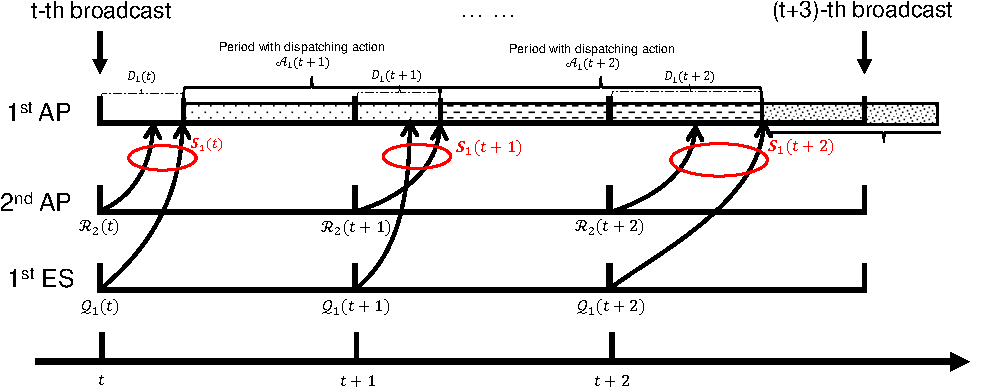
\includegraphics[width=0.60\textwidth]{brd-timeline.pdf}
    \caption{The timeline illustration of reception of OSI for the $1$-st AP where $2$-nd AP is in its \emph{conflict AP set} and $1$-st server is in its \emph{candidate server set}.}
    \label{fig:brd-timeline}
\end{figure*}

The $k$-th AP is able to collect its OSI at the $\mathcal{D}_{k}(t)$-th time slots of the $t$-th broadcast interval, where the \brlatency~$\mathcal{D}_{k}(t)$ is a random variable.
It is assumed that $\mathcal{D}_{k}(t)$ follows identical and independent distribution in different broadcast interval.
We refer to $\mathcal{D}_{k}(t)$ as the \brlatency~of the $k$-th AP at the $t$-th broadcast interval.
An example is given below to demonstrate how the \brlatency~affects the reception of OSI and the update of the dispatching strategy.

\begin{example}
    An example is illustrated in Fig.\ref{fig:brd-timeline}, where the $2$-nd AP and $1$-st server are in the \emph{conflict AP set} and \emph{candidate server set} of the $1$-st AP, respectively.
    At the beginning of the $t$-th broadcast interval, the dispatching actions $\mathcal{A}_{1}(t)$ is adopted by the $1$-st AP.
    Then after $\mathcal{D}_{1}(t)$ time slots, it updates the dispatching actions to $\mathcal{A}_{1}(t+1)$ based on the OSI.
    At the start of the $(t+1)$-th broadcast interval, it will firstly keep the previous actions, and then updates the actions immediately $\mathcal{D}_{1}(t+1)$ time slots later which is denotes as $\mathcal{A}(t+2)$.
    The signaling latency $\mathcal{D}_1(t)$ and $\mathcal{D}_1(t+1)$ can be different.
\end{example}
